%\documentclass[12pt]{scrreprt}
\documentclass[12pt]{report} 

% language may be romanian or english (default is english)
% type may be bachelor or master (default is bachelor)
\usepackage[language=english, type=bachelor]{style}

%\geometry{a4paper,top=2.5cm,left=3cm,right=2.5cm,bottom=2.5cm}
%in style
%controlling the appearance of your headers and footers
\usepackage{fancyhdr}
\pagestyle{fancy}
\lhead{}
\chead{}
\renewcommand{\headrulewidth}{0.2pt}
\renewcommand{\footrulewidth}{0.2pt}

\begin{document}

\specialization{COMPUTER-SCIENCE, ENGLISH}	
\title{Web Based Collaborative Content Viewing}					   
\author{Ciorbă Rareş-Nicolaie}											
\supervisor{Assoc. Prof. Rareș Florin Boian, PhD}				
				
\maketitle


\newpage
\thispagestyle{empty}
\mbox{}
\newpage
\pagenumbering{roman} 

\cleardoublepage
ABSTRACT

This thesis explores the problem that other web-based collaborative content viewing applications have: the simplicity of their permission system. In order to do this, the problem is thoroughly explained with real life examples in Chapter 2.

However the reason why most other applications have the problem of having a permission system that is too simple is because implementing an exhaustive permission system is a massive task and requires a lot of infrastructure and work. In order to do this properly, in Chapter 3, the thesis goes over different kind of access control mechanisms and tries to choose the best one to implement.

% Due to the fact that the thesis explores the topic of permission systems, it would be futile if the application is vulnerable from a security stand point, hence the application is split into front end and back end, and a secure connection is needed between those two. In Chapter 4, a thorough explanation of the technologies used to build the application is present.

% In Chapter 5, the thesis explains how the application implemented the actual access control mechanisms. In order to have a proper example of the control mechanism and permission system, the capability of having different users is needed alongside the actual control mechanism implementation, which chapter 5 glosses over. Finally, the thesis goes over how the mechanisms have been implemented and how a user would use the application to grant or remove access for users on the file structure they have.

Chapter 4 explores the application from beginning to end. An overview of the requirements is present as well as motivation behind picking all of the technologies that have been picked. After that the software requirements are explained as well as how the project is setup. Lastly, the implementation details and the usage of the application is explained.

Finally, the thesis ends with the Chapter 5, the conclusion and future work chapter, in which what has been learned from the thesis is explained as well as how the application could be further expanded.
\vspace{0.5cm}	
\hrule
\vspace{0.5cm}	
%\cleardoublepage


\tableofcontents


\newpage
\pagenumbering{arabic}

\chapter{Introduction}

%\chapter*{Introducere}
\label{intro}
% The topic of this thesis is to explore permissions control and security in a real-life 
% example such as a platform for content viewing. In order to facilitate an elaborate enough 
% permission control, Role-Based Access Control (RBAC) will be used. It will also explore .NET, 
% LINQ (SQL operations in .NET), JWT (JSON Web Tokens), React.js and Material UI.

% The primary purpose of this thesis is to provided a well-built application for sharing files
% in a web manner without compromising on security or the privacy of the hosted files. In order 
% to facilitate the security and privacy of the hosted files, the host of the application will 
% use an admin account which has total control over the permissions of its users. The admin 
% can provide default permissions for the default role, specific roles with specific permissions 
% --- for either files, folders or the application's settings and configurations.

\section{What is a permission system?}
To explain what a permission system is, firstly a need to understand what exactly a permission is exists. A permission is more or less a rule which is applied to either an object or an action. A permission system is a way of handling and managing the permissions, as well as putting them into use.
\section{Why are permission systems necessary?}
A permission system is necessary because it let's a user manage individual or group access and handle constraints around various objects, actions, users, or roles. In essence, a permission system has been in use for a very long time. The best example regarding a permission system is a file permission system.
\section{What is the purpose of this thesis?}
The purpose of this thesis is to provide an interactive and more exhaustive system of control in a web environment. The problem that this thesis is trying to address is that most collaborative content viewing solutions such as: Google Drive, or Dropbox explore very simplistic permissions. But because of their simplistic permission approach, a need for a very specific structure for files and folder is needed in other to facilitate a complete control over all of the data a user wants to share. 

Because the needs of a user and what they would want to share with other users will always change, having a very specific structure in mind for the files and folders becomes a big problem that becomes very chaotic and hard to manage. In order to solve this issue, this thesis proposes a more exhaustive permission system for the content of the user, that allows a lot more control.

\section{Thesis structure}
The thesis will contain an additional 5 chapters.
\begin{itemize}
    \item Permission implementation in other apps --- This chapter explores what other applications have done regarding their permission implementation, and why a more exhaustive permission control system might have advantages over the simplistic approaches of other applications.
    \item Permission management --- How exactly are permissions handled and what are the different ways of managing permissions by exploring two major attribute control systems --- ABAC and RBAC.
    \item The application --- This chapter explores how the application actually manages and solves the problem proposed in this thesis. What technologies it uses, and other technical details revolving around the app.
    \item Conclusions and Future work
\end{itemize}

%\addcontentsline{toc}{chapter}{Introduction}

\chapter{Permission implementations in other applications}
As previously mentioned, most implementations for permissions in other web based collaborative content viewing applications are too simplistic and don't provide the user with a complete control over the actions another user takes or the influence they can have on objects. 

\section{Google Drive}
One of the most popular systems for sharing files between users is Google Drive.
Google Drive introduces three ways of sharing a file or a folder with other users:
sharing via contact, sharing via a link, or publishing.

However, associated with these three types of sharing files or folders, a user can set three types of permissions on the files they wish to share: can edit, can view, or can comment. \cite{googleDrivePermission:1}

The "can edit" permission means that the user that gets access to the resource will be able to edit the content of the resource in its entirety.

The "can view" permission is just a read-only permission, thus the user is not allowed to modify the file or folder they have access to.

The "can comment" permission means that the user gets access to Google Drive's comment section and can leave comments regarding the contents of a document.

Although this system is very simple to use it comes with a few drawbacks. There are a few scenarios where sharing documents with the proper permission might cause be an issue. 

\begin{figure}[htbp]
	\centering
		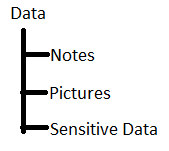
\includegraphics[scale=0.85]{./figures/chapter2/google_drive_file_structure.png}
	\caption{Hard to express file structure}
	\label{FigDriveBadScenario}
\end{figure}

Consider the file structure as shown in figure \ref{FigDriveBadScenario}, assume that the user wants to give access to the folder called "Data" to another user. Currently if the user wants to protect the folder called "Sensitive Data", the only way to do that would be to to share "Notes" and "Pictures" individually without exposing the whole "Data" folder. For this example doing that might work, but once we add a lot of other folders, the whole situation becomes very tedious.

\section{Unix systems}
Although not an online system, unix systems have a very good way of dealing with permissions which is worth going over. The core premise of the unix permission system is that permissions are divided into 3 actions: read, write, execute, along 3 subjects, the owner, the group and other users. 

Alongside all of these, unix systems also provide a so-called "god" role, the root role, which has access over every file and folder, and they can freely execute any command, which involves tinkering with the permissions of other users, groups, files, or folders. In actuality the "root" user is one of the most targeted place of attack, because if a malicious person gains access to the root account, they can do anything in the system.

The problem unix system have with their permission is, again, the lack of granularity. Even though they provide access for the owner, the group, and other users, the fact that you can only control access to one owner, and to one group can lead to issues.

\begin{figure}[htbp]
	\centering
		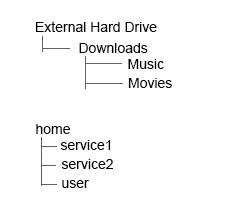
\includegraphics[scale=0.75]{./figures/chapter2/unix_file_structure.png}
	\caption{Complex file structure}
	\label{FigUnixBadScenario}
\end{figure}

Let's take the file structure expressed in \ref{FigUnixBadScenario} as an example. The system has 3 roles: a role for the user --- the owner of the system --- and 2 other roles representing services that are running on the system. Due to security reasons, the services run in their own separate roles.

\begin{table}[htbp]
	\begin{center}
		\begin{tabular}{|p{40pt}|p{220pt}|p{120pt}|}
			\hline User name  &  Access &  Description \\
			\hline 
			\hline user & Everything from the External Hard Drive & The user of the system \\
			\hline service1 & Music & - \\
			\hline service2 & Movies & - \\
			\hline
		\end{tabular}
	\end{center}
	\caption{User roles and permissions}
	\label{UnixRolesAndPerms}
\end{table}

Taking the permissions as described in \ref{UnixRolesAndPerms}, the first role, the user wants complete access ove the external hard drive. The second role, "service1" wants access to just the "Music" folder, without knowing about the existence of the "Movies" folder. And finally the third role "service2" wants access to the "Movies" folder without knowing about the existence of the "Music" folder. 

With just these three roles, the permission scheme proposed is easily achievable as described in \ref{UnixRolesAndPerms2}.
\begin{table}[htbp]
	\begin{center}
		\begin{tabular}{|p{80pt}|p{80pt}|p{80pt}|p{50pt}|}
		\hline Folder & Owner & Group & Other \\
		\hline
		\hline External HDD & user - rw & user - rw & - \\
		\hline Music & user - rw & service1 - rw & - \\
		\hline Movies & user - rw & service2 - rw & - \\
		\hline
		\end{tabular}
	\end{center}
	\caption{User roles and permissions}
	\label{UnixRolesAndPerms2}
\end{table}

The first column represents the folder. The second column represents who the owner is, and the "rw" represents that they have read write access. The third column represents what the group is, and the "rw", again represents that they have read write access. For the sake of example and simplicity the "execute" permission will be left out. The other column represents what permissions other users have, i.e the ones that aren't the owner or are part of the group.

With this permission schema, the user, being the owner of the "External HDD" folder has access over it and all of its subfolders. The role "service1" has access to the "Music" folder, but because the "Music" folder has no read or write permission specified for "others" that means that it can not be accessed by "service2". The same idea was applied to the "Movies" folder, and for the role "service2". 

Even though this is a fairly simple example, the structure of the permission system is a bit cluttered and hard to manage, but in the end it does represent the file structure aforementioned.

The problem with this rises once we introduce more users and more folders.

\begin{figure}[htbp]
	\centering
		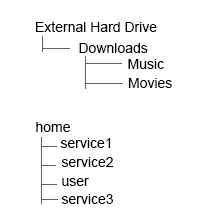
\includegraphics[scale=0.75]{./figures/chapter2/unix_file_structure_2.png}
	\caption{Example bad scenario for unix}
	\label{FigUnixBadScenario2}
\end{figure}

As shown in figure \ref{FigUnixBadScenario2}, the file structure remains the same but a single role has been added. In this case the role "service3" can be seen as a file sharing service such as sambashare. The role "service3" requires complete access over the whole directory that is "Downloads", but no other directories on the External Hard Drive.

Due to the fact that the unix system provides control over a single role, a single owner, and all other users, there is no way of achieving this file structure, and this permission structure, without having to change the structure of the files.

\chapter{Permission management}
\label{chap:ch1}

In order for the application to provide the necessary security over files a permission system
needs to be implemented. There are various ways of implementing permissions, two fairly used 
techniques are Attribute-based access control (ABAC) and Role-based access control (RBAC).
\section{Attribute-based access control}
Attribute-based access control (ABAC) is an authorization model that evaluates attributes 
(or characteristics), rather than roles, to determine access.\cite{keithABAC} The purpose of this 
attribute-based authorization model is to preserve the security and integrity of data 
or devices by restricting access only to authorized users. 

\begin{figure}[htbp]
	\centering
		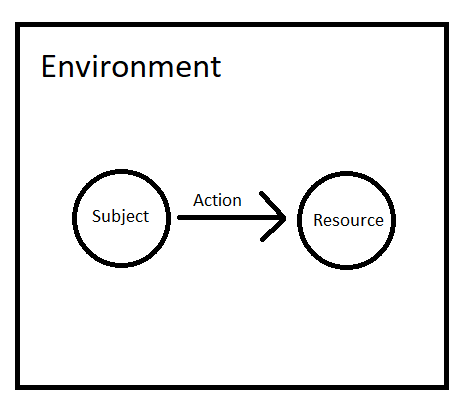
\includegraphics[scale=0.65]{./figures/chapter3/abac.png}
	\caption{The 4 major components of ABAC}
	\label{FigABAC}
\end{figure}


ABAC contains 4 major components: Subject, Resource, Action, and Environment as seen in \ref{FigABAC}.

Although the subject of ABAC is usually associated with a user, in reality,
the Subject can be either a role, a user profile, or essentially any identifying
criteria. Generally, the Subject is identified by their authentication token, 
for example even something like the Personal Numeric Code can be used. 

The Resource is an asset or an object --- be it a file, an application, 
a server or an API --- that the Subject wants to access. 

The Action represents what the Subject wants to perform on the Resource. 
A good example for the Actions is the common actions a file explorer can perform: read, 
write, edit, copy, delete. An Action can have multiple attributes (parameters) 
associated with it. For example, a copy could have the source and the destination.

The Environment represents the context in which the Action has been performed. 
The context can contain data such as: the date and the time when the action was 
performed, the location from which the Subject is trying to perform the Action, 
or even the communication protocol or information about the encryption strength.

Attributes are the characteristics involved during an access event. Attribute-based
access control analyzes these attributes against a set of rules in order to determine
if the subject is authorized.

\subsection*{Advantages}
The key benefit of ABAC is its flexibility. Essentially, the limit for policy-making lies in what attributes must be accounted for, and the conditions the computational language can express. ABAC allows for the greatest breadth of subjects to access the greatest amount of resources without requiring admins to specify relationships between each subject and object. Take the following steps as an example:

\begin{itemize}
    \item When a subject joins an organization, they're assigned a set of subject attributes (e.g., John Doe is a consultant for the radiology department).
    \item An object, when created, is assigned its attributes (e.g., a folder with cardiac imaging test files for heart patients).
    \item  The admin or object owner then creates an access control rule (e.g., "All consultants for the radiology department can view and share cardiac imaging test files for heart patients").
\end{itemize}

Admins can further modify these attributes and access control rules to fit the needs of an organization. For instance, when defining new access policies for external subjects like contractors and providers, they can do so without manually changing each subject-object relationship. ABAC allows for a wide variety of access situations with little administrative oversight.
\subsection*{Disadvantages}
ABAC can be difficult to get off the ground. Admins need to manually define attributes, assign them to every component, and create a central policy engine that determines what attributes are allowed to do, based on various conditions (“if X, then Y”). The model's focus on attributes also makes it hard to gauge the permissions available to specific users before all attributes and rules are in place.\cite{keithABAC}

However, while implementing ABAC can take considerable time and resources, the effort does pay off. Admins can copy and reuse attributes for similar components and user positions, and ABAC's adaptability means that maintaining policies for new users and access situations is a relatively “hands-off” affair.

\section{Role-based access control}

Role-based access control (RBAC) is an authorization model where the roles are the only ways to determine the access to a certain resource or action. A certain simplicity in the ABAC idea is appealing. If a user has attributes that are reflected in the objects they want to access, then access is granted. On the other hand, with RBAC, the permissions granted to a user through roles must be evaluated to determine if the desired access will be granted.\cite{coyneABAC}

\subsection*{Advantages}
Unlike ABAC, where each individual users has a set of attributes, with RBAC all users are assigned a role, which makes the management of the permissions for a set of users easier to manage. Other key benefits of RBAC include:

\begin{itemize}
	\item The possibility of creating a re-assignable sets of permissions.
 	\item Reduce the risk of human error when assigning permissions. 
  	\item Granularity of permissions is still preserved by breaking up permissions into multiple roles and assigning multiple roles to users.
	\item Reduce administrative work by having the possibility of quickly changing the user's roles (i.e after a project ends and an user access needs to be revoked).
 	\item Decrease the security risks by restricting access to sensitive information in a more controlled manner.
\end{itemize}

\subsection*{Disadvantages}
Despite having a simpler implementation compared to ABAC, RBAC does of course come with disadvantages. The main disadvantage of RBAC is that due to the increasing number of different roles, managing said roles becomes a very complex task if the management wishes to have properly encapsulated permissions.

Granularity is also much harder to achieve than with an ABAC system. In the case where you want only a user to have a privilege and that user is part of a group already, the only way to give that user and only that user the privilege is to create a new role solely for that.
\chapter{The application}
\section{Overview of the requirements}
As mentioned in the 2nd chapter of the thesis, one of the major problems in many applications that revolve around permissions is the fact that they don't provide a granular enough system. In order to deal with this, unlike the Google Drive, the demo application must implement an exhaustive system, and unlike unix systems, the application must allow multiple roles to be assignable to a single user.

In order to achieve this the application must have the following features:
\begin{itemize}
    \item A user system, and therefore the ability to switch between the perspective of different users.
    \item A way of managing roles: assigning roles to users, changing permissions of the roles, adding/removing roles.
    \item And finally, a way of actually testing the permissions out in a realistic environment.
\end{itemize}

\section{Backend --- used technologies}
\subsection{.NET and C\#}
.NET is a free, cross-platform and open source framework developed by Microsoft, that started as proprietary. The reason .NET was chosen for this application is because it provides an environment for building very expandable Rest APIs. 

One of the key benefits of .NET core is Entity Framework Core. Entity Framework (EF) Core is a lightweight, extensible, open source and cross-platform version of the popular Entity Framework data access technology.

EF Core can serve as an object-relational mapper (O/RM), which\cite{efCore}:

\begin{itemize}
 	\item Enables .NET developers to work with a database using .NET objects. \item Eliminates the need for most of the data-access code that typically needs to be written.
\end{itemize}

EF Core supports many database engines such as SQLite, PostgreSQL, MySQL, etc.
\subsection{LINQ}
LINQ or Language integrated query is the name for a set of technologies based on integrating SQL-like queries straight into C\#, which has the benefit of compile-time checking rather than runtime. Writing SQL code as a set of string is very error prone and fairly hard to manage, and LINQ helps to alleviate that problem.

To do that, LINQ provides SQL-specific keywords such as \verb|from|, \verb|where|, \verb|select| which can be used on collections as shown in figure \ref{FigLINQExample}.

\begin{figure}[htbp]
	\centering
		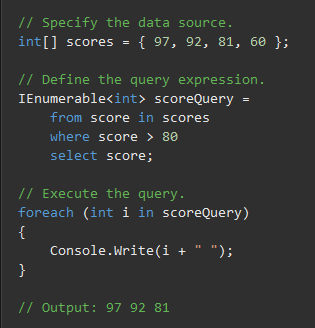
\includegraphics[scale=0.85]{./figures/chapter4/linq_example.png}
	\caption{LINQ Example}
	\label{FigLINQExample}
\end{figure}

The LINQ system further contributed to the choice of using .NET for the application, since there were a lot of interconnected entities.

\subsection{JSON Web Token}
Even though the scope of this thesis is to explore the permission management in an application focused on collaborative content viewing, it would all be futile if the application is easily exploitable through security vulnerabilities, and thus a need for a secure and encrypted means of communication between the front end and the back end exists.

The JSON Web Token or JWT for short is a proposed internet standard for creating data with optional signature and/or optional encryption whose payload holds JSON that asserts some number of claims.
\section{Frontend --- used technologies}
\subsection{React.js}
React (also known as React.js or ReactJS) is a free and open-source front-end Java-Script library for building user interfaces based on UI components. It is maintained by Meta (formerly Facebook) and a community of individual developers and companies.

React is component based which allows the user to build encapsulated components that manage their own state, and then further compose them into a more complex user interface.

React also makes it painless to create interactive UIs. Design simple views for each state in your application, and React will efficiently update and render just the right components when your data changes. \cite{reactJs}

Declarative views make your code more predictable and easier to debug.

\subsection{Typescript}
TypeScript is a programming language developed and maintained by Microsoft. It is a strict syntactical superset of JavaScript and adds optional static typing to the language. It is designed for the development of large applications and transpiles to JavaScript. As it is a superset of JavaScript, existing JavaScript programs are also valid TypeScript programs. 

TypeScript provides static typing through type annotations to enable type checking at compile time. This is optional and can be ignored to use the regular dynamic typing of JavaScript. 

Because Typescript provides typing, developing becomes overall easier as code is much easier to debug since you won't rely on runtime errors to spot bugs, but instead, the code fails at compile time.

\subsection{Material UI}
The main reason react was chosen lies within the material ui library. MUI is a ReactJS library that provides components based on the Material UI standard developed by Google. It allows a quick and easy way of developing responsive applications without the need of worrying about the aesthetic of the application.

The components that it provides also come with a lot of functionality by default which further saves time during development.


\section{Software Requirements}
In order to run both the projects, an operating system is needed. Due to the fact that the backend project uses .NET, the software requirements regarding the operating system are mostly given by it. Hence a machine with an operating system that can run dotnet CLI at minimum is needed. 

Known supported operating systems include\cite{dotnetSupportedOs}:
\begin{itemize}
    \item Windows and Windows server
    \item MacOS
    \item Linux and linux servers: Ubuntu, Alpine, CentOS, Debian, etc.
\end{itemize}

For the frontend the major dependency is React.js, in order to install that Node.js is needed. 

The operating system requirements for nodejs are pretty much the same as the ones for dotnet\cite{nodejsSupportedOs}:
\begin{itemize}
    \item Windows
    \item MacOS
    \item Linux: Ubuntu, Debian, CentOS, etc.
\end{itemize}

Since both projects are essentially source code that needs to be compiled, an IDE (Integrated Development Environment) is strongly recommended for both of them.

For the backend project there are many different choices: Rider, Visual Studio, Visual Studio Code. As for the frontend project, any IDE that has support for html, css, typescript should suffice, for example InteliJ, PhpStorm, WebStorm, Visual Studio Code, Sublime Text.

During the development phase, I used Rider for the backend and PhpStorm for the front end, which I strongly recommend as that is what will be used to explain the setup and running of the projects.

\section{Setup}
Since the application is split into two different projects, each one of them needs to be set up individually.
\subsection{Backend}
The backend is written in C\# with .NET framework core. The first requirement is to have dotnet installed. After that the app settings need to be configured. To do that, navigate to \verb|Backend/Backend|, and copy paste the template file called \verb|appsettings.template.json| into another file called \verb|appsettings.json|.

\begin{figure}[htbp]
	\centering
		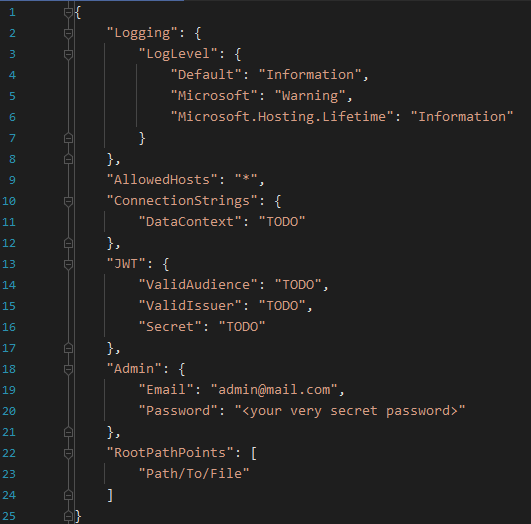
\includegraphics[scale=0.85]{./figures/chapter4/appsettings_template.png}
	\caption{App settings template}
	\label{FigAppSettingsTemplate}
\end{figure}

Next, as shown in figure \ref{FigAppSettingsTemplate}, a few fields need to be filled. The first field is related to the \verb|ConnectionStrings|. A ConnectionString is a way of specifying how to connect the application to the database. During development, the database used was SQLite. 

To specify a connection to that set \verb|DataContext| equal to \\ \verb|"Data Source=<Location>;"|, where Location will be the location of the \\ database. 

Example: \verb|"DataContext":  "Data Source=Kumo.db;"|.

The second field that needs to be configured is related to the JSON Web Token  (JWT). The ValidAudience represents the location at which the requests with the token will be valid. For example if you want to have only one computer use the API, then the IP address of that computer will become the ValidAudience, meanwhile in the case where anybody can be a valid audience, the field is set to \verb|*|. Next, the ValidIssuer represents the location from which the token can be created. This is always the address associated with the server.

The final and the most important field from the JWT configuration is the \verb|Secret|. This represents a base64 encoded string which is used for creating the token. If this field is not secure enough, or it gets leaked, then the JWT becomes reversible, which is why this field is extremely important to remain a secret.

The third field that needs to be configured is related to the Admin. Normally having an endpoint that creates an administrator user is bad practice, which is why the application handles this by providing a way of creating the administrator user at the first start of the application. The \verb|Email| and \verb|Password| fields are explanatory.

The fourth field is related to the Root Path Points. In short, a root path point is a place from which the navigation can start. This field is not mandatory as these can be created from the front end, via the administrator account.

After setting up the \verb|appsettings.json| file, the next step is to create the database and all of the schema for it. To do that, we need to run migrations which require a dependency called \verb|dotnet-ef|. 

To install \verb|dotnet-ef|, a few commands need to be run. The first one being \verb|dotnet tool install --global dotnet-ef|. After that we can create the database, to do that you need to be in the same directory as the \verb|appsettings.json| file, and then run \verb|dotnet ef database update|.

With that, all the setting up for the back end is finished, and the backend is now runnable.

Open your IDE of choice, in this case Rider will be used. Simply open the project in it, and hit the \verb|Run| button in the top right corner.

\begin{figure}[htbp]
	\centering
		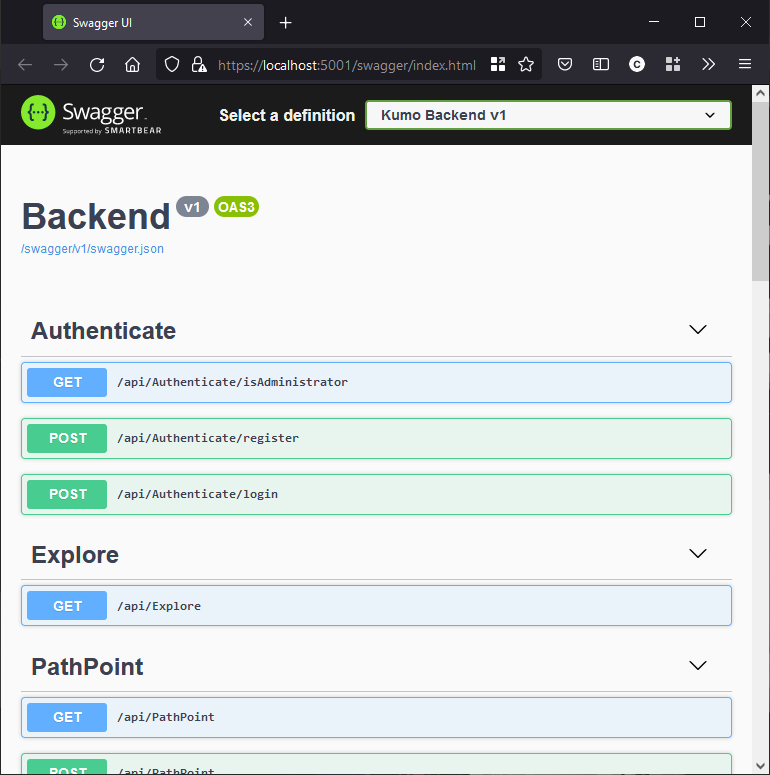
\includegraphics[scale=0.6]{./figures/chapter4/backend_swagger.png}
	\caption{Swagger and the API endpoints}
	\label{FigBackendSwagger}
\end{figure}

After that, you should see Swagger, like shown in the figure \ref{FigBackendSwagger}.

\subsection{Frontend}
Compared to the backend project, setting up the frontend is significantly easier, as only two commands need to be run. After navigating to the \verb|frontend| directory, we need to install the dependencies. To do that simply open a terminal and write \verb|npm install|.

After that completes, open your IDE of choice, in this case PhpStorm will be used. Open the project in it and then run it via the \verb|Run| button.

\begin{figure}[htbp]
	\centering
		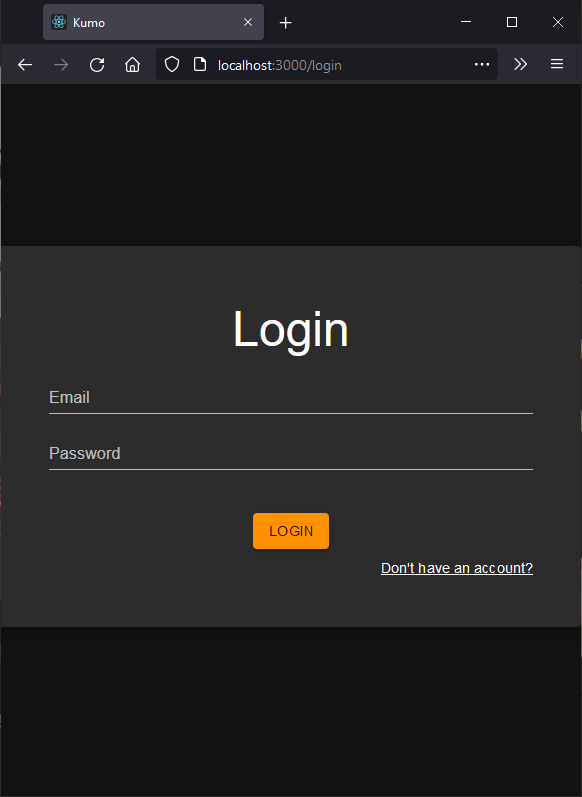
\includegraphics[scale=0.5]{./figures/chapter4/frontend_login.png}
	\caption{Frontend login page}
	\label{FigFrontendLogin}
\end{figure}

Once the application has finished compiling, a browser will open and you will see a login screen, as shown in \ref{FigFrontendLogin}.


\section{Implementation details}
The implementation of the application uses RBAC, hence a way of managing roles is needed. This however starts with correctly separating the data in the database to make different operations possible and to account for different use cases.

To do this the data is structures into 6 classes:
\begin{itemize}
	\item PathPoint --- represents a specific location, has one important property: \verb|isRoot|. \verb|isRoot| represents if the path should be displayed on the explorer's home page;
 	\item FileSystemEntryType --- an enum that specifies if the system entry type is a file or a folder, or unknown;
	\item Role --- self explanatory, it represents a role;
	\item Permission --- this is an n:m relation between a PathPoint and a Role, with additional data such as: Read, Write, Delete;
	\item User --- this represents a user in the application;
 	\item UserRole --- this is an n:m relation between a User and a Role.
\end{itemize}

\section{Application usage}
As mentioned in the requirements, in order to explore the problem of permissions, 3 main functionalities are needed. A way of managing users, a way of managing permissions, and a real life usage of those permission.
\subsection{Users}
Thus, the first requirement the application must have is a way of handling users. The application has functionality for register\ref{FigFrontendRegister}, login\ref{FigFrontendLogin}, and logout marked with a (1) in \ref{FigFrontendLogout}.

\begin{figure}[htbp]
	\centering
		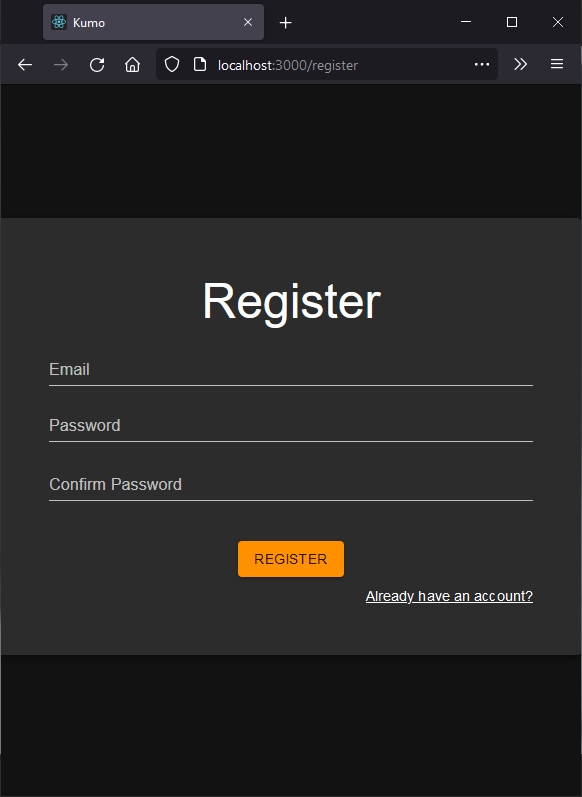
\includegraphics[scale=0.5]{./figures/chapter4/frontend_register.png}
	\caption{Frontend register page}
	\label{FigFrontendRegister}
\end{figure}

\begin{figure}[htbp]
	\centering
		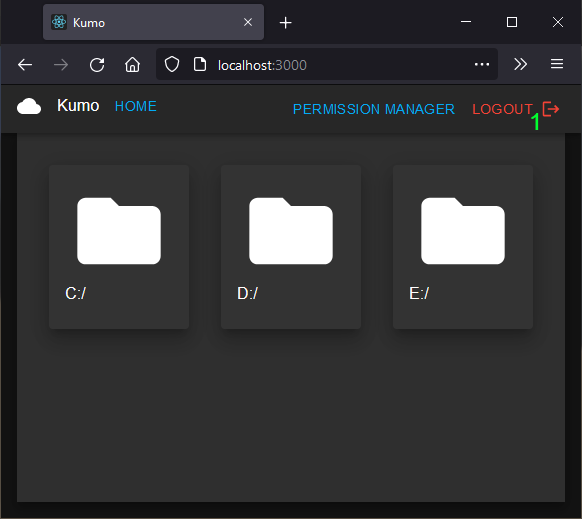
\includegraphics[scale=0.5]{./figures/chapter4/frontend_logout.png}
	\caption{Frontend logout functionality on the main page}
	\label{FigFrontendLogout}
\end{figure}

Being trivial functionality, there is no reason to go over the flow of each of the actions.
\subsection{Explorer}
The real life usage of the permissions is an Explorer. The explorer, essentially, provides a way of navigating folders on a hard drive.

Being used as a proof of concept, the main purpose of the explorer is to give a visual representation of how the "Read" permission works across all instances where it has been set. Due to the fact that the permission system takes into account permissions such as "Delete" and "Write", the Explorer can be easily expanded to accommodate for those too, however for the sake of example the Read permission will be used as a visual representation, while the response from the API calls will contain more information.

\begin{figure}[htbp]
	\centering
		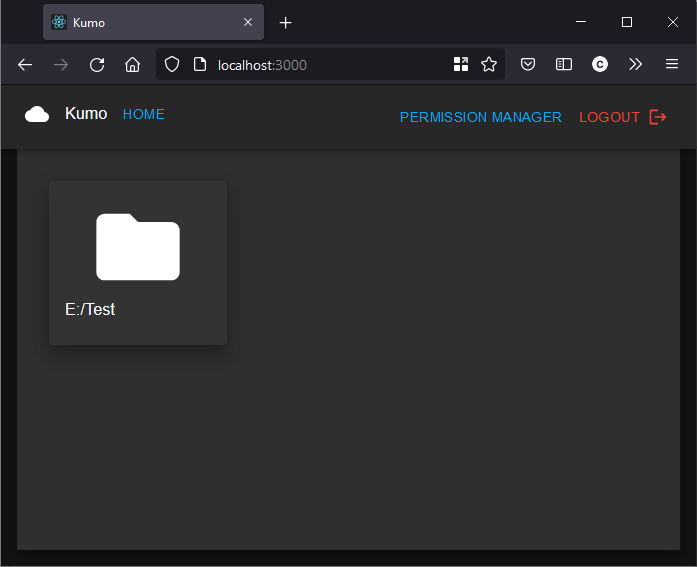
\includegraphics[scale=0.65]{./figures/chapter4/explorer_home.png}
	\caption{Explorer home path}
	\label{FigExplorerHome}
\end{figure}

\begin{figure}[htbp]
	\centering
		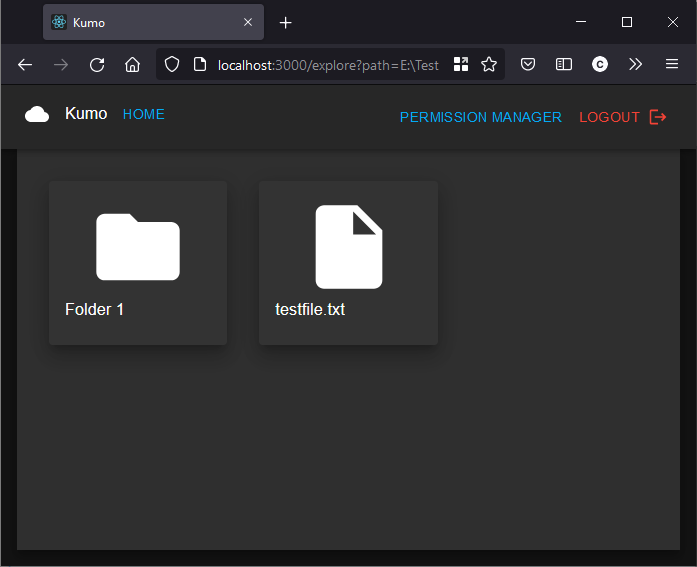
\includegraphics[scale=0.65]{./figures/chapter4/explorer_subfolder.png}
	\caption{Explorer subfolder navigation}
	\label{FigExplorerSubFolder}
\end{figure}

As mentioned in the implementation details, on the explorer home page\ref{FigExplorerHome} the root path points are shown. When a user clicks on a directory, the explorer moves inside that subdirectory and shows the files and folders inside it. When clicking on the \verb|E:/Test| subfolder it's contents are shown as in \ref{FigExplorerSubFolder}.

\subsection{Permission management}
The most important part of the application is the permission management system. As mentioned in Setup of the Backend, an admin account is needed. To properly show the functionality of this, I'm going to use two browsers which are connected to two accounts. As shown in \ref{FigPermissionManagerButton}, the browser on the left is connected to an admin account, which shows the \verb|PERMISSION MANAGER| button, while the browser on the right doesn't.

\begin{figure}[htbp]
	\centering
		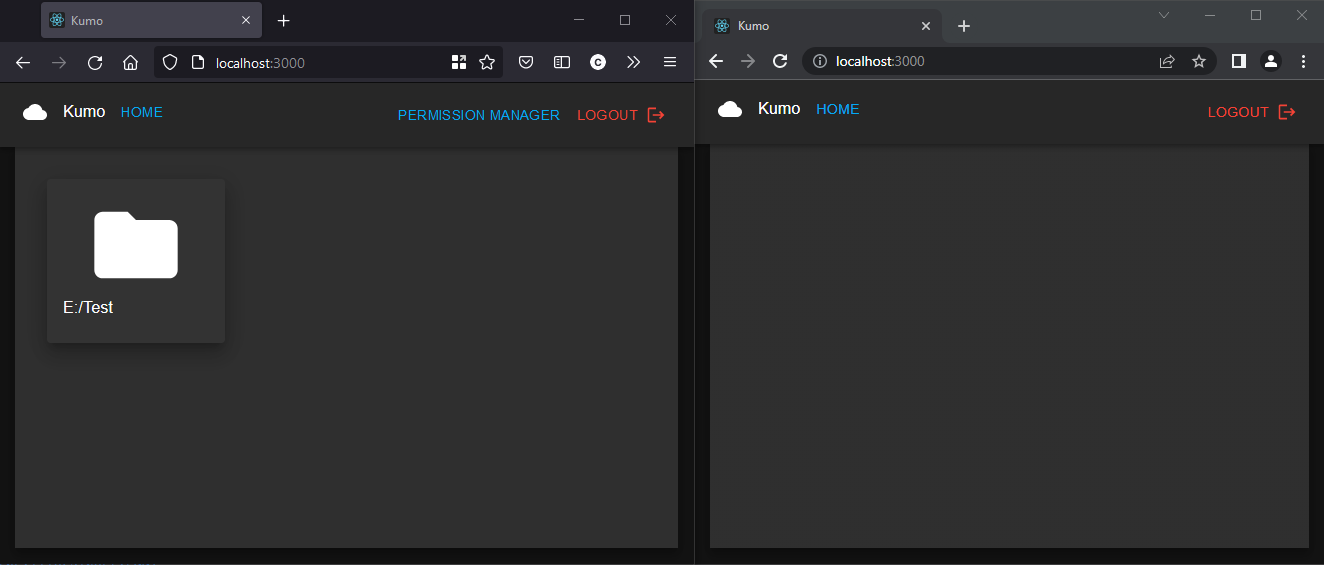
\includegraphics[scale=0.4]{./figures/chapter4/explorer_permission_manager.png}
	\caption{Permission manager button on an admin account and on an normal account}
	\label{FigPermissionManagerButton}
\end{figure}


You'll notice that in figure \ref{FigPermissionManagerButton}, the user on the right does not see any path points. And that is because there are no permissions configured yet aside from the \verb|E:/Test| path point.

To configure the permissions, the first step is to go to the Permission Manager. Due to the complexity of the permission manager, there are 4 configurable entries as shown in figure \ref{FigPermissionManagerHome}

\begin{figure}[htbp]
	\centering
		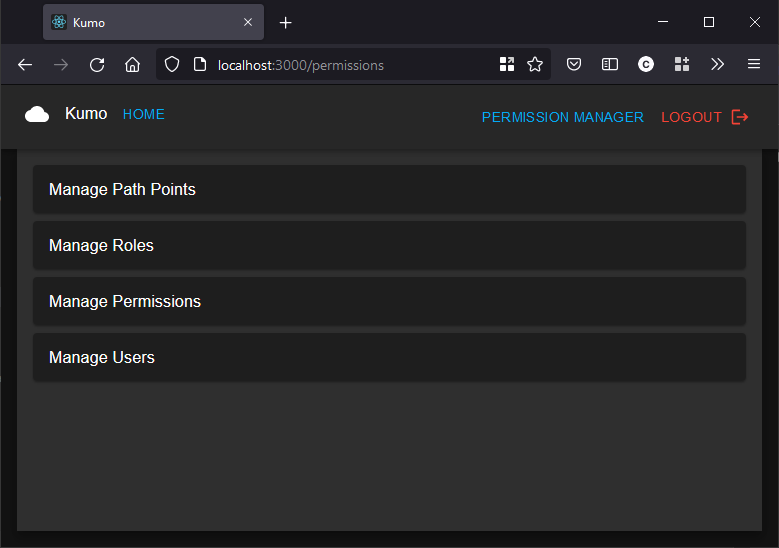
\includegraphics[scale=0.6]{./figures/chapter4/permission_manager_home.png}
	\caption{The default view of the permission manager}
	\label{FigPermissionManagerHome}
\end{figure}

To demonstrate the power of the permission system, we will configure the scenario mentioned in chapter 2, the hard to express file structure from google drive shown in figure \ref{FigDriveBadScenario}.

\subsubsection{Configuring Path Points}
Once you click on the \verb|Manage Path Points| button, the accordion will expand and the path point manager will be shown as in figure \ref{FigPermissionManagerPathPoints}

Firstly, all managers have a table that show the entries available in the database. In the case of the Path Point Manager, there are a number of important elements:
\begin{itemize}
	\item (1) --- Shows the path of the path point
	\item (2) --- Shows whether or not the path point is root
	\item (3) --- Marks the entry for deletion
	\item (4) --- Commits the changes from the table to the database
	\item (5) --- Cancels all of the changes and reverts to the original state from the database
	\item (6) --- The path of the new path point to be added
	\item (7) --- Whether or not the path point is a root path point
	\item (8) --- Adds the path point to the database
\end{itemize}

Entries (1) and (2) can be edited by double clicking on them.

To achieve the file structure mentioned, where the Sensitive Data isn't accessible by a user, a path point that is not a root is needed for the \verb|Sensitive Data| folder as shown in figure \ref{FigPermissionManagerPathPointsCorrect}.

\begin{figure}[htbp]
	\centering
		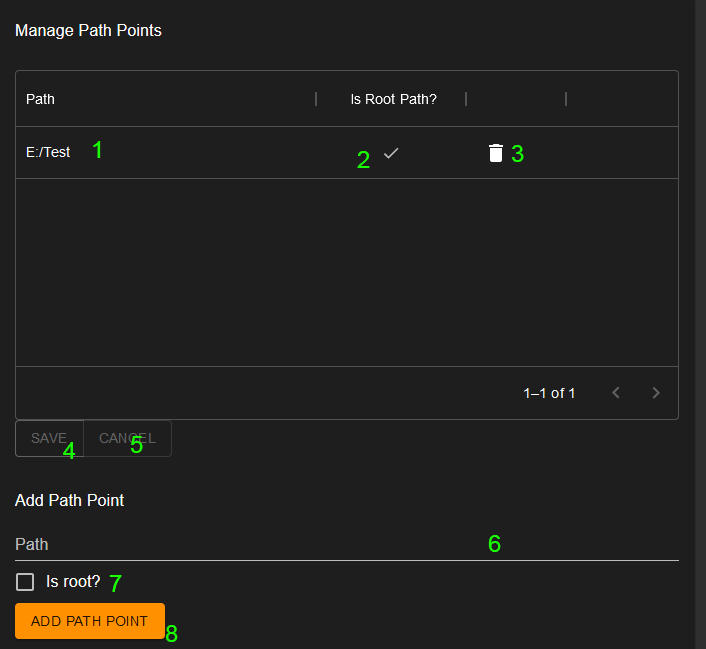
\includegraphics[scale=0.5]{./figures/chapter4/permission_manager_path_points.png}
	\caption{Path point manager}
	\label{FigPermissionManagerPathPoints}
\end{figure}


\begin{figure}[htbp]
	\centering
		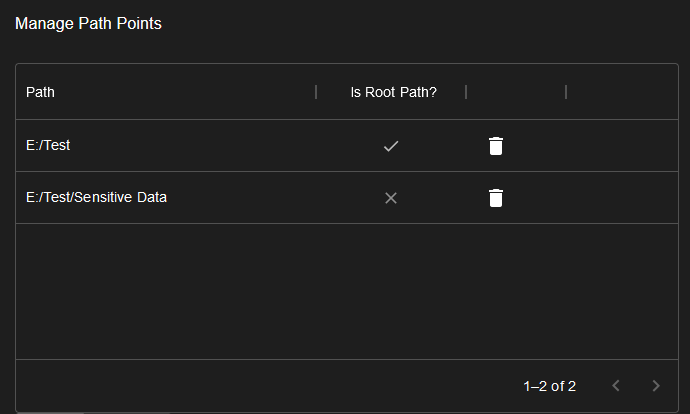
\includegraphics[scale=0.65]{./figures/chapter4/permission_manager_correct_path_points.png}
	\caption{The correct path point structure needed}
	\label{FigPermissionManagerPathPointsCorrect}
\end{figure}

\subsubsection{Configuring Roles}
To achieve the desired permission structure only one role is needed, to do that configure it by opening the role manager as shown in \ref{FigPermissionManagerRoles}.

The important elements in the role manager are as follows:
\begin{itemize}
	\item (1) --- The name of the role;
	\item (2) --- Marks the element for deletion;
	\item (3) --- Commits the changes from the table to the database;
	\item (4) --- Cancels all of the changes and reverts to the original state from the database;
	\item (5) --- The name of the role to be added;
	\item (6) --- Adds the role to the database.
\end{itemize}

\begin{figure}[htbp]
	\centering
		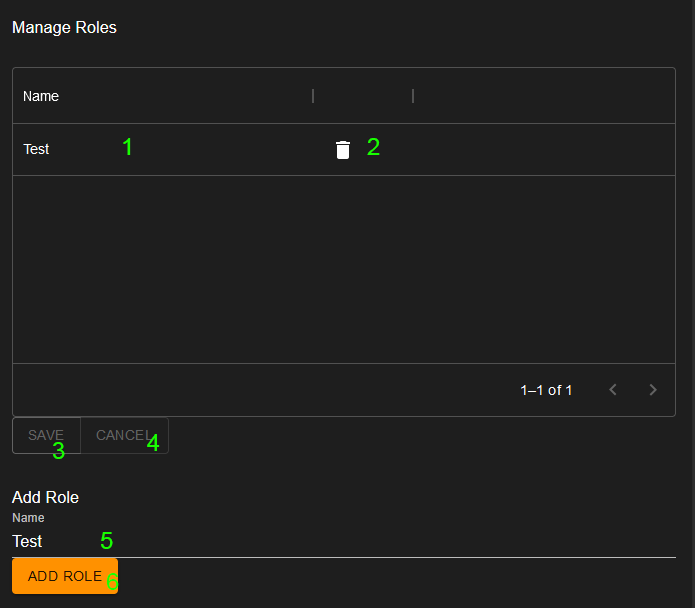
\includegraphics[scale=0.5]{./figures/chapter4/permission_manager_roles.png}
	\caption{Roles manager}
	\label{FigPermissionManagerRoles}
\end{figure}

\subsubsection{Configuring Permissions}
For configuring permissions we essentially need to specify that the \verb|E:/Test| path is readable by the \verb|Test| role, and the \verb|E:/Test/Sensitive Data| is not readable by the \verb|Test| role.

As marked in figure \ref{FigPermissionManagerPermission}, the important elements are as follows:
\begin{itemize}
	\item (1) --- The role for which the permission is applied;
	\item (2) --- The path for which the permission is applied;
	\item (3), (4), (5), (6) --- Whether or not the role can: Modify Root, Read, Write, or Delete;
	\item (7) --- Marks the element for deletion;
	\item (8) --- Commits the changes from the table to the database;
	\item (9) --- Cancels all of the changes and reverts to the original state from the database;
	\item (10) --- The role of the new permission
	\item (11) --- The path point for the new permission
	\item (12), (13), (14), (15) ---  Whether or not the new role can: Modify Root, Read, Write, or Delete;
	\item (16) --- Adds the permission to the database.
\end{itemize}

\begin{figure}[htbp]
	\centering
		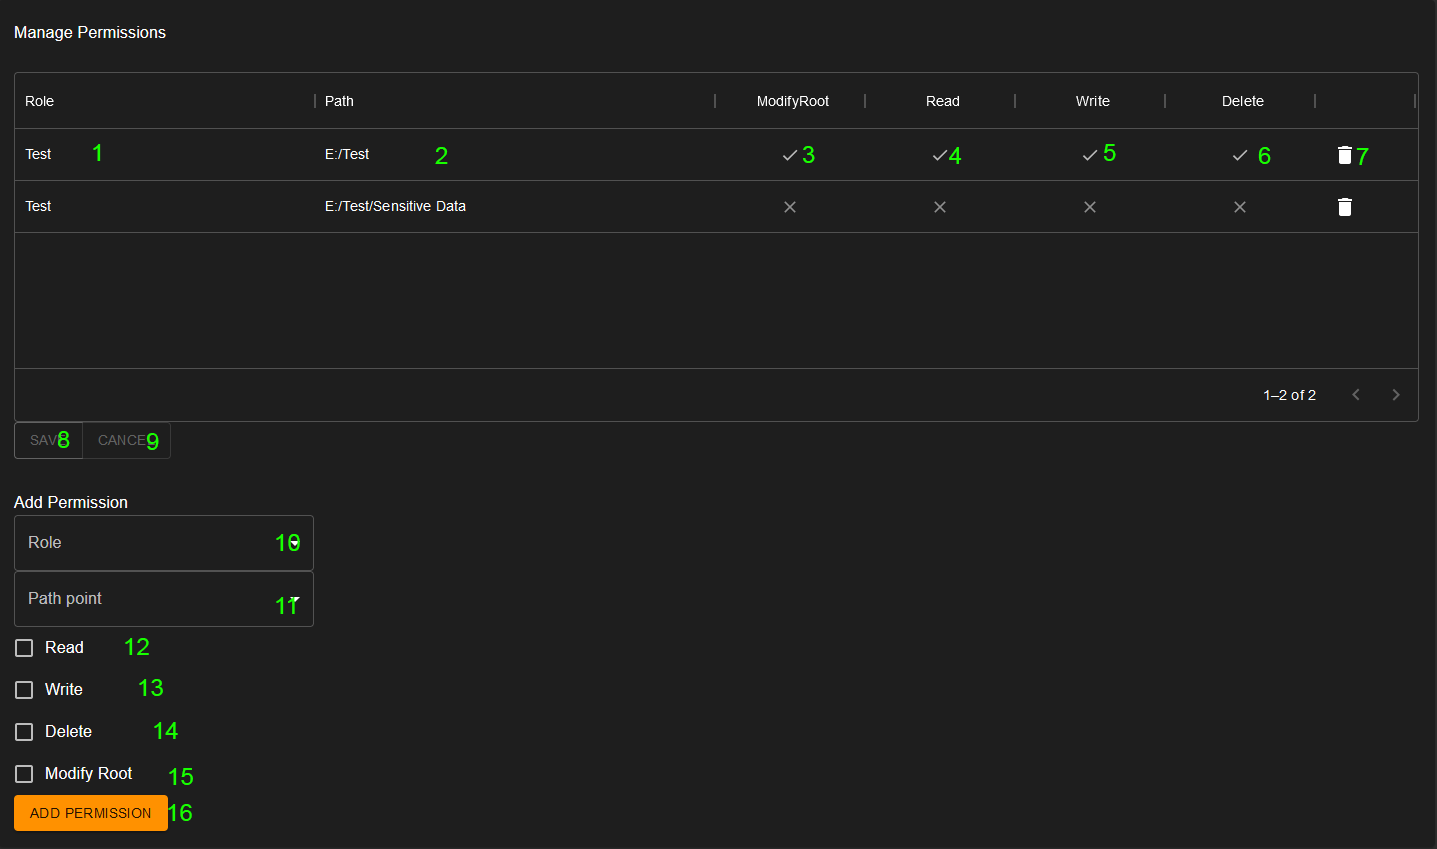
\includegraphics[scale=0.3]{./figures/chapter4/permission_manager_permission.png}
	\caption{Permission manager}
	\label{FigPermissionManagerPermission}
\end{figure}


\subsubsection{Configuring Users}
The last step is to connect the \verb|test@mail.com| user to the \verb|Test| role.

As marked in figure \ref{FigPermissionManagerUser}, the important elements are as follows:
\begin{itemize}
	\item (1) --- The user that is linked;
	\item (2) --- The role to which the user is linked;
	\item (3) --- Marks the element for deletion;
	\item (4) --- Commits the changes from the table to the database;
	\item (5) --- Cancels all of the changes and reverts to the original state from the database;
	\item (6)--- The user that will be linked;
	\item (7) --- The role the user will be linked to;
	\item (8) --- Links the user to the role in the database.
\end{itemize}

\begin{figure}[htbp]
	\centering
		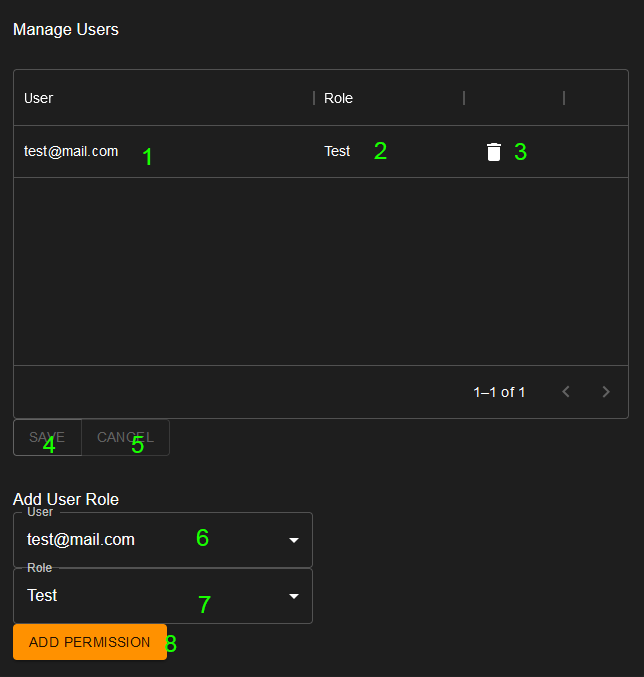
\includegraphics[scale=0.5]{./figures/chapter4/permission_manager_users.png}
	\caption{User manager}
	\label{FigPermissionManagerUser}
\end{figure}

With that all of the configuration has been done, if the user \verb|test@mail.com| navigates to the \verb|E:/Test| path, they will be unable to see the \verb|Sensitive Data| directory, as shown in figure \ref{FigPermissionManagerResult}.


\begin{figure}[htbp]
	\centering
		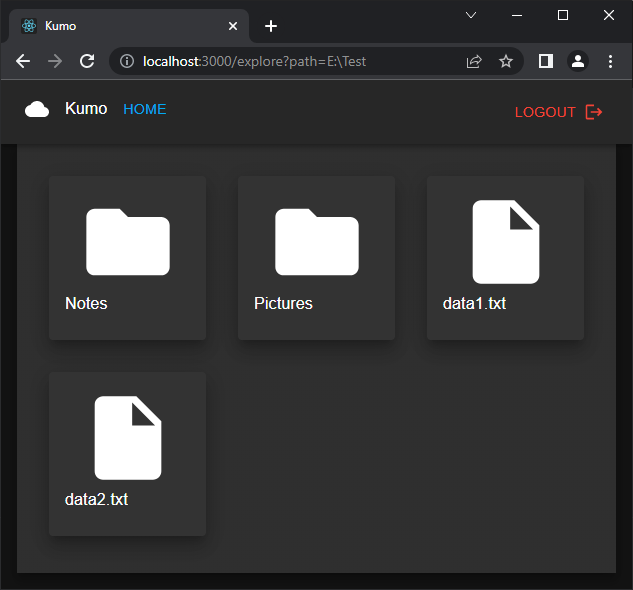
\includegraphics[scale=0.65]{./figures/chapter4/permission_manager_result.png}
	\caption{Permission manager result in the explorer}
	\label{FigPermissionManagerResult}
\end{figure}
\input{chapters/chapter5}

\chapter{Conclusions and Future Work}
\label{conclusions}

\section*{Conclusion}
The complexity that was unachievable with Google Drive or Unix systems mention in Chapter 2 is completely achievable by implementing a Role-based attribute control system. Of course, with the increased complexity problems also arise. The "Role explosion" problem mentioned in Chapter 3 remains an issue because in order to achieve proper granularity, a lot of roles will be needed.


\section*{Future work}
With the application being a proof of concept, a lot of new features could be added to it. The explorer could be easily expanded by adding multiple views, more actions, and by overall offering more control over the navigation, files, and folders. 

Due to the fact that the backend was written in C\#, expanding the permission object is fairly easy as only a database migration is needed which is easily achievable with just a few commands.

Currently, there is only one role that can modify permissions, but allowing users to modify permissions in a hierarchy would also be possible. For example if a user has access to a specific directory, they can further modify the permissions of the subdirectories of that directory. But this of course comes with new challenges as the new system would become fairly cluttered and even harder to manage and to implement. 

%\addcontentsline{toc}{chapter}{Conclusions}

\bibliography{references}
\end{document}
